\maketitlesupplementary

% Sections are lettered; figures, tables, and equations continue the numbering of the submitted main paper
% (which ends at Figure 8, Table 3, and Eq. (11)).
\setcounter{figure}{8}\setcounter{table}{3}\setcounter{equation}{11}
\setcounter{section}{0}\renewcommand{\thesection}{\Alph{section}}
% \planned{...}: outline text for a part that is not written yet; remove the macro's uses before submission.
\raggedbottom  % columns end where the text ends; the kit's \flushbottom stretched short paragraphs apart
\renewcommand{\qedsymbol}{}  % no end-of-proof square; proofs end with a sentence
\newcommand{\planned}[1]{{\color{blue!60!black}\textit{[Planned] #1}}}

This supplementary material is organized as follows. \Cref{sec:supp-proofs} provides the derivations and proofs omitted from the main paper. \Cref{sec:supp-impl} lists the implementation details and hyperparameters. \Cref{sec:supp-exp} reports the sensitivity analysis and additional experiments.

\section{Derivations and Proofs}
\label{sec:supp-proofs}

For completeness, we restate the allocation problem of the main paper. Let $b_i\in[0,b_i^{\max}]$ be the tokens allocated to item $i\in\mathcal F\cup\mathcal S$, with token value $v_i(b_i)=b_i/(b_i+\tau_i)$, where $\tau_i$ is $\tau_{\text{frame}}$ for a frame and $\tau_{\text{text}}$ for a subtitle. \name solves
\begin{equation}
\begin{aligned}
  \max_{\mathbf b}\quad & \sum_{i\in\mathcal F} r_i(q,\mathbf b)\,v_i(b_i)+\beta\sum_{i\in\mathcal S} r_i(q,\mathbf b)\,v_i(b_i)\\
  \text{s.t.}\quad & \sum_{i\in\mathcal F\cup\mathcal S} b_i\le B ,
\end{aligned}
\label{eq:supp-allocation}
\end{equation}
where the allocation-dependent relevance discounts the retrieval relevance $r_i(q)$ by the token values of the similar items of the same modality $\mathcal M_i\in\{\mathcal F,\mathcal S\}$:
\begin{equation}
  r_i(q,\mathbf b)=r_i(q)-\eta\sum_{j\in\mathcal M_i}s_{ij}\,v_j(b_j) .
\label{eq:supp-cond}
\end{equation}

\paragraph{Setup.}
All proofs in this section use the same few quantities. Each item $i$ has a token count $b_i$ and a token value $z_i=v_i(b_i)\in[0,1)$; we write $\mathbf b$ and $\mathbf z$ for the vectors of all items. $\mathcal Z$ is the set of token values that respect the budget, and $J(\mathbf z)$ is the objective of \cref{eq:supp-allocation} written in token values (both defined in \cref{sec:supp-convex}). The gradient $\nabla J(\mathbf z)$ is the discounted relevance of the main paper. Finally, $L=2\eta\,\sigma_{\max}$ measures the curvature of $J$, where $\sigma_{\max}$ is the largest eigenvalue of the similarity matrix $\mathbf S$, and $D$ is the largest distance between two points of $\mathcal Z$.

\subsection{Convexity of the Continuous Relaxation}
\label{sec:supp-convex}

We first show that, after a change of variables, the relaxed problem maximizes a concave function over a convex set. Every later result relies on this property. We change variables from token counts to token values $z_i=v_i(b_i)$. Since $v_i$ is strictly increasing, this change of variables is invertible, with
\begin{equation}
  b_i=v_i^{-1}(z_i)=\frac{\tau_i z_i}{1-z_i} ,
\label{eq:supp-inverse}
\end{equation}
where $0\le z_i\le z_i^{\max}=v_i(b_i^{\max})<1$.
The feasible set of token values under the budget $B$ is, therefore,
\begin{equation}
  \mathcal Z=\Big\{\mathbf z:\ 0\le z_i\le z_i^{\max},\ \ \sum_{i}\frac{\tau_i z_i}{1-z_i}\le B\Big\} .
\label{eq:supp-feasible}
\end{equation}
Each function $\tau_i z_i/(1-z_i)$ is convex on $[0,1)$, because its second derivative $2\tau_i/(1-z_i)^3$ is positive. The budget constraint thus bounds a sum of convex functions, and $\mathcal Z$ is convex and compact.

Substituting \cref{eq:supp-cond} into \cref{eq:supp-allocation} expresses the objective in terms of the token values as
\begin{equation}
  J(\mathbf z)=\bar{\mathbf r}^{\top}\mathbf z-\eta\,\mathbf z^{\top}\mathbf S\mathbf z ,
\label{eq:supp-quadratic}
\end{equation}
where $\bar r_i=r_i(q)$ for a frame and $\bar r_i=\beta\,r_i(q)$ for a subtitle, and $\mathbf S$ is block-diagonal with the frame similarity matrix and the $\beta$-scaled subtitle similarity matrix as its blocks. Each block contains the cosine similarities between the embeddings of one modality, including the diagonal entries $s_{ii}=1$. It is, therefore, the Gram matrix of the normalized embeddings and is positive semidefinite. Since $\beta>0$ and $\eta\ge0$, the matrix $\eta\,\mathbf S$ is positive semidefinite and $J$ is concave. Maximizing $J$ over $\mathcal Z$ is thus a convex program, and every local maximum is a global maximum~\cite{boyd2004}.

\subsection{Derivation of Water-Filling}
\label{sec:supp-waterfill}

Consider the subproblem with fixed relevances $\bar r_i>0$:
\begin{equation}
\begin{aligned}
  \max_{\mathbf b}\quad & \sum_i \bar r_i\,\frac{b_i}{b_i+\tau_i}\\
  \text{s.t.}\quad & \sum_i b_i\le B,\quad 0\le b_i\le b_i^{\max} .
\end{aligned}
\label{eq:supp-fixed}
\end{equation}
We derive its solution through the Lagrangian dual. The idea is to replace the budget by a price per token, let each item buy tokens at that price, and then adjust the price until the budget is spent. Introducing a multiplier $\lambda\ge0$ for the budget constraint, and keeping the bounds $0\le b_i\le b_i^{\max}$ as the domain of $\mathbf b$, gives the Lagrangian
\begin{equation}
  \mathcal L(\mathbf b,\lambda)=\sum_i \bar r_i\,\frac{b_i}{b_i+\tau_i}-\lambda\Big(\sum_i b_i-B\Big) .
\label{eq:supp-lagrangian}
\end{equation}
The subproblem equals $\max_{\mathbf b}\min_{\lambda\ge0}\mathcal L(\mathbf b,\lambda)$, and its dual is $\min_{\lambda\ge0}\max_{\mathbf b}\mathcal L(\mathbf b,\lambda)$. Since the objective is concave, the constraints are linear, and $\mathbf b=\mathbf 0$ is strictly feasible, strong duality holds~\cite{boyd2004}: the two problems attain the same value, and a maximizer of $\mathcal L(\cdot,\lambda^\star)$ at the dual optimum $\lambda^\star$ that meets the budget solves the subproblem.

\paragraph{Inner maximization.}
For a fixed $\lambda>0$, the Lagrangian separates over the items, and each item solves
\begin{equation}
  \max_{0\le b_i\le b_i^{\max}}\ \bar r_i\,\frac{b_i}{b_i+\tau_i}-\lambda\,b_i .
\label{eq:supp-item}
\end{equation}
Intuitively, $\lambda$ acts as a price per token, and each item acquires tokens until its marginal gain falls to this price. The objective of \cref{eq:supp-item} is strictly concave, so setting its derivative to zero,
\begin{equation}
  \frac{\bar r_i\,\tau_i}{(b_i+\tau_i)^2}=\lambda ,
\label{eq:supp-stationarity}
\end{equation}
and clipping the solution to the domain yields its unique maximizer
\begin{equation}
  b_i(\lambda)=\left[\sqrt{\bar r_i\tau_i/\lambda}-\tau_i\right]_0^{b_i^{\max}} ,
\label{eq:supp-waterfill}
\end{equation}
which is the water-filling allocation of the main paper. In particular, an item receives no tokens when its marginal gain at zero tokens, $\bar r_i/\tau_i$, does not exceed $\lambda$, and it receives its full token count when its marginal gain at $b_i^{\max}$ is at least $\lambda$. An item with $\bar r_i\le0$ cannot increase the objective and receives no tokens.

\paragraph{Outer minimization.}
Substituting \cref{eq:supp-waterfill} into \cref{eq:supp-lagrangian} gives the dual function $g(\lambda)=\mathcal L(\mathbf b(\lambda),\lambda)$, which is convex in the single variable $\lambda$ with derivative
\begin{equation}
  g'(\lambda)=B-\sum_i b_i(\lambda) .
\label{eq:supp-dual}
\end{equation}
If $\sum_i b_i^{\max}\le B$, the budget is not binding and every item receives its full token count. Otherwise, the dual optimum $\lambda^\star$ satisfies $g'(\lambda^\star)=0$, i.e., the allocation spends exactly the budget. Because of the clipping, this equation has no closed-form solution in general. However, each $b_i(\lambda)$ is continuous and non-increasing in $\lambda$, and all of them vanish once $\lambda\ge\max_i\bar r_i/\tau_i$, so a bisection over $\lambda\in(0,\max_i\bar r_i/\tau_i]$ finds $\lambda^\star$. Since each term of \cref{eq:supp-fixed} with $\bar r_i>0$ is strictly concave, the resulting allocation $\mathbf b(\lambda^\star)$ is the unique maximizer.

\subsection{Proof of Proposition 1}
\label{sec:supp-convergence}

\noindent\textbf{Proposition 1} (restated)\textbf{.} \textit{Let $J^\star$ be the global maximum of \cref{eq:supp-allocation} over continuous token allocations, and let $J^{(\ell)}$ be the objective value after $\ell$ iterations of iterative water-filling. Then}
\begin{equation}
  J^\star-J^{(\ell)}\le\frac{4\,\eta\,\sigma_{\max}D^2}{\ell+2} .
\label{eq:supp-rate}
\end{equation}

The proof follows the standard analysis of the Frank--Wolfe method~\cite{jaggi2013} and uses two ingredients. The first bounds how far the current allocation is from the optimum. The second bounds how much one iteration improves the objective.

\begin{lemma}[Distance to the optimum]
\label{lem:gap}
For every $\mathbf z\in\mathcal Z$,
\begin{equation}
  J^\star-J(\mathbf z)\le\max_{\mathbf y\in\mathcal Z}\,\nabla J(\mathbf z)^{\top}(\mathbf y-\mathbf z) .
\label{eq:supp-lem-gap}
\end{equation}
\end{lemma}
\begin{proof}
Let $\mathbf z^{\rm opt}$ be a maximizer of $J$ over $\mathcal Z$. Since $J$ is concave, its linear approximation at $\mathbf z$ lies above it, so $J^\star=J(\mathbf z^{\rm opt})\le J(\mathbf z)+\nabla J(\mathbf z)^{\top}(\mathbf z^{\rm opt}-\mathbf z)$. The right-hand side is at most the maximum over all $\mathbf y\in\mathcal Z$.
\end{proof}

\noindent Intuitively, the best improvement predicted by the linear approximation is never smaller than the true remaining gap. The maximization on the right of \cref{eq:supp-lem-gap} is exactly what one water-filling pass solves: in token values, the objective of \cref{eq:supp-fixed} with relevances $\nabla J(\mathbf z)$ is the linear function $\nabla J(\mathbf z)^{\top}\mathbf y$, and its constraints define $\mathcal Z$.

\begin{lemma}[Progress of one step]
\label{lem:step}
For every $\mathbf z,\mathbf s\in\mathcal Z$ and $\gamma\in[0,1]$,
\begin{equation}
\begin{aligned}
  J\big(\mathbf z+\gamma(\mathbf s-\mathbf z)\big)\ge{}& J(\mathbf z)+\gamma\,\nabla J(\mathbf z)^{\top}(\mathbf s-\mathbf z)\\
  &-\frac{L}{2}\gamma^2D^2 .
\end{aligned}
\label{eq:supp-lem-step}
\end{equation}
\end{lemma}
\begin{proof}
Write $\mathbf d=\gamma(\mathbf s-\mathbf z)$. Since $J$ is quadratic, its second-order expansion is exact: $J(\mathbf z+\mathbf d)=J(\mathbf z)+\nabla J(\mathbf z)^{\top}\mathbf d-\eta\,\mathbf d^{\top}\mathbf S\mathbf d$. The last term is at least $-\eta\,\sigma_{\max}\|\mathbf d\|^2=-\frac{L}{2}\|\mathbf d\|^2$, and $\|\mathbf d\|\le\gamma D$.
\end{proof}

\noindent In words, a step of size $\gamma$ toward $\mathbf s$ gains the improvement predicted by the linear approximation, minus a curvature penalty that shrinks with $\gamma^2$.

\begin{proof}[Proof of Proposition 1]
We first show that each iteration removes a fixed fraction of the remaining gap, and then solve the resulting recursion by induction. Let $\mathbf z^{(\ell-1)}$ be the token values before iteration $\ell$, with $\mathbf z^{(0)}=\mathbf 0$, and let $h_\ell=J^\star-J(\mathbf z^{(\ell)})$ be the remaining gap. Iteration $\ell$ runs water-filling with the discounted relevance $\nabla J(\mathbf z^{(\ell-1)})$, which returns the maximizer $\mathbf s$ of the right-hand side of \cref{eq:supp-lem-gap}, and moves to $\mathbf z^{(\ell)}=\mathbf z^{(\ell-1)}+\gamma_\ell(\mathbf s-\mathbf z^{(\ell-1)})$ with $\gamma_\ell=2/(\ell+1)$. This point lies in $\mathcal Z$ because $\mathcal Z$ is convex.

Our starting point is \cref{lem:step} with $\mathbf z=\mathbf z^{(\ell-1)}$ and $\gamma=\gamma_\ell$:
\begin{align*}
  J(\mathbf z^{(\ell)})
  &\ge J(\mathbf z^{(\ell-1)})+\gamma_\ell\,\nabla J(\mathbf z^{(\ell-1)})^{\top}(\mathbf s-\mathbf z^{(\ell-1)})\\
  &\qquad-\frac{L}{2}\gamma_\ell^2D^2\\
  &\ge J(\mathbf z^{(\ell-1)})+\gamma_\ell\,h_{\ell-1}-\frac{L}{2}\gamma_\ell^2D^2 ,
\end{align*}
where the second line uses \cref{lem:gap}. Subtracting both sides from $J^\star$ gives
\begin{equation}
  h_\ell\le(1-\gamma_\ell)\,h_{\ell-1}+\frac{L}{2}\gamma_\ell^2D^2 .
\label{eq:supp-recursion}
\end{equation}
This contraction relates the gap after an iteration to the gap before it: each iteration removes a fraction $\gamma_\ell$ of the gap, at the price of a curvature term.

We now show $h_\ell\le2LD^2/(\ell+2)$ by induction. For $\ell=1$, the step size is $\gamma_1=1$, and \cref{eq:supp-recursion} gives $h_1\le LD^2/2\le2LD^2/3$. For $\ell\ge2$, assume the claim for $\ell-1$, i.e., $h_{\ell-1}\le2LD^2/(\ell+1)$. Then
\begin{align*}
  h_\ell&\overset{\text{(a)}}{\le}\frac{\ell-1}{\ell+1}\,h_{\ell-1}+\frac{2LD^2}{(\ell+1)^2}\\
  &\overset{\text{(b)}}{\le}\frac{\ell-1}{\ell+1}\cdot\frac{2LD^2}{\ell+1}+\frac{2LD^2}{(\ell+1)^2}\\
  &=\frac{2LD^2\,\ell}{(\ell+1)^2}\overset{\text{(c)}}{\le}\frac{2LD^2}{\ell+2} ,
\end{align*}
where (a) substitutes $\gamma_\ell=2/(\ell+1)$ into \cref{eq:supp-recursion}, (b) applies the induction hypothesis, and (c) uses $\ell(\ell+2)\le(\ell+1)^2$. Substituting $L=2\eta\,\sigma_{\max}$ gives \cref{eq:supp-rate}, which completes the proof.
\end{proof}

\noindent Two remarks help interpret the bound. First, the constant grows with $\eta$: a stronger redundancy penalty couples the items more and requires more iterations. Without the penalty ($\eta=0$), the bound is zero, and the first iteration, plain water-filling, is already optimal. Second, the bound applies to the continuous allocation, before it is rounded down to whole tokens. Since every token value lies in $[0,1)$, the diameter satisfies $D^2\le|\mathcal F|+|\mathcal S|$.

\subsection{Suboptimality of Prior Allocation Rules}
\label{sec:supp-prior}

The main paper states that neither proportional allocation~\cite{luo2025quota} nor tiered allocation~\cite{zhang2025qframe} maximizes the fixed-relevance objective of \cref{eq:supp-fixed}. We make both statements precise.

\begin{lemma}[Proportional allocation]
\label{lem:proportional}
Suppose at least three items have pairwise distinct relevances $\bar r_i>0$ and share the same parameter $\tau$, and let $b_i=c\,\bar r_i$ with $c>0$ satisfy $0<b_i<b_i^{\max}$ for these items. Then this allocation does not maximize \cref{eq:supp-fixed}.
\end{lemma}
\begin{proof}
By \cref{sec:supp-waterfill}, an optimal allocation requires all items with $0<b_i<b_i^{\max}$ to share the same marginal gain, i.e., $\bar r_i\tau/(c\,\bar r_i+\tau)^2=\lambda$ for some $\lambda>0$. Rearranged, every such relevance is a root of the quadratic $\lambda c^2x^2+(2\lambda c\tau-\tau)x+\lambda\tau^2=0$ in $x$. A quadratic has at most two distinct roots, which contradicts the three pairwise distinct relevances.
\end{proof}

\noindent Intuitively, proportional allocation would equalize the marginal gains only if the value of an item grew like $\log b_i$, a value that never saturates. With a saturating value, it keeps adding tokens to the most relevant items after their value has saturated, and takes these tokens from less relevant items that would still benefit.

\begin{lemma}[Tiered allocation]
\label{lem:tiered}
Suppose two items of the same tier have distinct relevances $\bar r_i\ne\bar r_j$, share the same parameter $\tau$, and receive the same token count $b$ with $0<b<\min(b_i^{\max},b_j^{\max})$. Then this allocation does not maximize \cref{eq:supp-fixed}.
\end{lemma}
\begin{proof}
An optimal allocation requires equal marginal gains for the two items, $\bar r_i\tau/(b+\tau)^2=\bar r_j\tau/(b+\tau)^2$, which holds only if $\bar r_i=\bar r_j$.
\end{proof}

\noindent Intuitively, the more relevant of the two items still gains more from its next token, so moving one token to it raises the objective.

In both cases, the water-filling allocation of \cref{eq:supp-waterfill} is the unique maximizer and, therefore, attains a strictly higher objective within the same budget.

\section{Implementation Details}
\label{sec:supp-impl}

\subsection{Settings of \name}
\label{sec:supp-settings}

\Cref{tab:supp-hparams,tab:supp-hparams-ivl} list the settings of \name with Qwen3-VL-8B~\cite{bai2025qwen3vl} and InternVL3.5-4B~\cite{wang2025internvl35}, respectively. The two encoders score the relevance of frames and subtitles to the query. The token value parameter $\tau$ sets how quickly the value $v_i(b_i)=b_i/(b_i+\tau_i)$ of an item saturates with tokens, and is fitted by least squares to the validation measurements of the main paper. The subtitle weight $\beta$ scales the relevance of subtitles against that of frames, and the redundancy penalty $\eta$ weighs the similarity between items that both receive tokens. Iterative water-filling runs for $L$ iterations, each of which finds the token price $\lambda$ by bisection. In multi-turn conversations, the attention weight $\omega$ controls how much the VLM's attention refines the relevance of cached items. The token budget $B$ is not a fixed setting: it controls the compute of each experiment and is stated with each result.

\begin{table}[t]
  \centering
  \footnotesize
  \renewcommand{\arraystretch}{1.15}
  \begin{tabular}{l l}
    \toprule
    Setting & Value \\
    \midrule
    Frame relevance encoder & SigLIP 2 (so400m-patch14-384)~\cite{siglip2} \\
    Subtitle relevance encoder & BGE (base-en-v1.5)~\cite{bge} \\
    Token value parameter $\tau_{\text{frame}}$ & 38 \\
    Token value parameter $\tau_{\text{text}}$ & 13.6 \\
    Subtitle weight $\beta$ & 0.5 \\
    Redundancy penalty $\eta$ & $2.67\times10^{-5}$ \\
    Iterations $L$ & 20 \\
    Bisection steps per iteration & 60 \\
    Attention weight $\omega$ & 0.5 \\
    \bottomrule
  \end{tabular}
  \caption{Settings of \name with Qwen3-VL-8B.}
  \label{tab:supp-hparams}
\end{table}

\begin{table}[t]
  \centering
  \footnotesize
  \renewcommand{\arraystretch}{1.15}
  \begin{tabular}{l l}
    \toprule
    Setting & Value \\
    \midrule
    Frame relevance encoder & SigLIP 2 (so400m-patch14-384)~\cite{siglip2} \\
    Subtitle relevance encoder & BGE (base-en-v1.5)~\cite{bge} \\
    Token value parameter $\tau_{\text{frame}}$ & 38 \\
    Token value parameter $\tau_{\text{text}}$ & 13.6 \\
    Subtitle weight $\beta$ & 0.5 \\
    Redundancy penalty $\eta$ & $2.67\times10^{-5}$ \\
    Iterations $L$ & 20 \\
    Bisection steps per iteration & 60 \\
    \bottomrule
  \end{tabular}
  \caption{Settings of \name with InternVL3.5-4B.}
  \label{tab:supp-hparams-ivl}
\end{table}

\subsection{VideoRAG Implementation}
\label{sec:supp-videorag}

We build on the released code of VideoRAG~\cite{ren2025videorag}, with Qwen3-VL-8B~\cite{bai2025qwen3vl} in place of GPT-4o-mini and MiniCPM-V. For each question, the frames of the clips that VideoRAG retrieves form the candidate frames, and its retrieved text chunks enter the prompt within the token budget. The VideoRAG row splits the budget equally across these frames, whereas \name allocates it.

\section{Additional Experiments}
\label{sec:supp-exp}

\subsection{Sensitivity Analysis}
\label{sec:supp-sens}

\name has three hand-set settings: the attention weight $\omega$ of attention refinement, the subtitle weight $\beta$, and the temperature $T$ of the softmax that turns the query similarities of the candidate items into the relevance $r_i(q)$. \Cref{fig:supp-omega,fig:supp-beta,fig:supp-T} vary each of them while keeping all other settings fixed. Every $\omega>0$ improves over retrieval relevance alone ($\omega=0$) in both accuracy and compute, and the values $\omega>0$ differ by less than one point. With $\beta=0$, no subtitle receives tokens and the prompt contains none, which reduces accuracy by 12 points, while all values $\beta>0$ stay within 2 points of each other. Accuracy is highest at the default temperature and drops by about 3 points when $T$ is much smaller or larger. \name is, therefore, robust to $\omega$ and $\beta$ within a wide range, and $T$ only needs to avoid the extremes.

\begin{figure}[t]
  \centering
  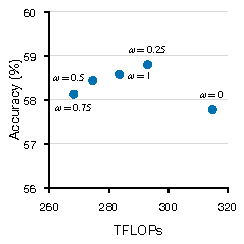
\includegraphics[width=\linewidth]{fig/sens_omega.pdf}
  \caption{Sensitivity of \name to the attention weight $\omega$ on MT-Video-Bench.}
  \label{fig:supp-omega}
\end{figure}

\begin{figure}[t]
  \centering
  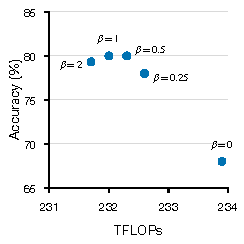
\includegraphics[width=\linewidth]{fig/sens_beta.pdf}
  \caption{Sensitivity of \name to the subtitle weight $\beta$ on Video-MME.}
  \label{fig:supp-beta}
\end{figure}

\begin{figure}[t]
  \centering
  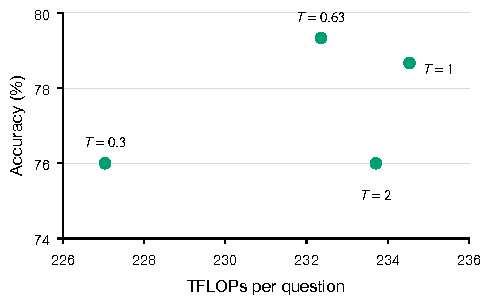
\includegraphics[width=\linewidth]{fig/sens_T.pdf}
  \caption{Sensitivity of \name to the relevance temperature $T$ on Video-MME.}
  \label{fig:supp-T}
\end{figure}

\subsection{Solver Efficiency}
\label{sec:supp-solver}

We compare iterative water-filling against two integer solvers, Gurobi~\cite{gurobi} and SCIP~\cite{scip}, which solve the discrete allocation problem to optimality, and against CVXPY~\cite{cvxpy} with the Clarabel solver~\cite{clarabel}, which solves the same continuous relaxation as iterative water-filling. We use synthetic videos of 30 to 3,600 candidate frames and a time limit of 10 minutes. As shown in \cref{tab:supp-solver}, iterative water-filling is 1.3--7$\times$ faster than CVXPY and 4--27$\times$ faster than Gurobi, while SCIP does not finish beyond 420 frames. Its objective stays within 0.04\% of the integer optimum.

\begin{table}[t]
  \centering
  \footnotesize
  \setlength{\tabcolsep}{3.4pt}
  \renewcommand{\arraystretch}{1.15}
  \begin{tabular}{r r r r r r}
    \toprule
    \multirow{2}{*}{Frames} & \multicolumn{4}{c}{Solving time (s)} & \multirow{2}{*}{Speedup} \\
    \cmidrule(lr){2-5}
    & Gurobi~\cite{gurobi} & SCIP~\cite{scip} & CVXPY~\cite{cvxpy} & Ours & \\
    \midrule
    30    & 0.04 & 1.9   & 0.010 & 0.006 & 1.8--349$\times$ \\
    60    & 0.03 & 4.0   & 0.013 & 0.007 & 1.8--539$\times$ \\
    120   & 0.09 & 9.7   & 0.039 & 0.009 & 4.3--1,061$\times$ \\
    240   & 0.20 & 23.9  & 0.040 & 0.031 & 1.3--771$\times$ \\
    420   & 0.56 & 51.7  & 0.080 & 0.025 & 3.2--2,060$\times$ \\
    1,800 & 3.01 & $>$600 & 0.76 & 0.13  & 5.8--$>$4,500$\times$ \\
    3,600 & 5.03 & $>$600 & 1.79 & 0.26  & 7.0--$>$2,300$\times$ \\
    \bottomrule
  \end{tabular}
  \caption{Solving time of iterative water-filling and three off-the-shelf solvers. Speedup ranges from the fastest to the slowest solver.}
  \label{tab:supp-solver}
\end{table}

